\section{Интернет вещей: сущность, основные подходы}
\label{sec:subject}

Индустрия электронного светового оборудования представляет обширную часть рынка продуктов в сфере развлечения. Ежегодно люди тратят много времени для украшения собственных домов. Различные компании вкладывают большие усилия и значительные финансовые средства для подготовки к различным праздникам, так как это может поспособствовать привлечению большого потока клиентов.

Однако сам процесс настройки и управления световым оборудованием на данный момент представляет собой очень простую, лишенную возможностей для пользовательских настроек, операцию. Чаще всего он заключается в простой смене доступных анимаций, путем нажатия на кнопку, расположенную на самом оборудовании.

Дипломный проект призван улучшить процесс взаимодействия пользователя с данным оборудованием (адресной светодиодной лентой). С помощью мобильного приложения и больших возможностей светодиодной ленты пользователи получат возможности для полноценной работы с светодиодной лентой: от создания собственных анимаций, до отправки их другим пользователям.

В данной главе будет рассмотрена история возникновения электронного светового оборудования и её взаимосвязь с понятием \enquote{Интернет вещей}, сущность Интернета вещей и основные подходы к реализации, взаимодействие мобильных приложений с устройствами в Интернете вещей, а также алгоритм распознавания расположения адресной светодиодной ленты в нашем приложении.

\subsection{Индустрия электронного светового оборудования}
\label{sec:subject:industry}

Электронное световое оборудование~--- это последовательность из сопряженных световых элементов, например светодиодов, под управлением какого-либо электронного устройства.

Начиная с конца 19-го века, когда русский электротехник Павел Николаевич Яблочков изобрел первую электрическую лампочку, и по сегодняшний день, индустрия электронного светового оборудования постоянно увеличивается в размерах. Разнообразие товаров растет, на рынке присутствует большой спрос, но и такая же большая конкуренция. Множество компаний получают контракты на освещение больших архитектурных сооружений, поставку светового оборудования для проведения различных музыкальных концертов (светомузыка) и так далее. Сама индустрия дистрибуции электронного светового оборудования ориентируется как на рынок физических лиц (украшения на елку, комнатное освещение, внешние украшения для дома), так и на юридических лиц (внешнее и внутренне освещение офисов, светомузыка, световые скульптуры). 

Рынок домашнего освещения становится все более и более популярным, особенно зарубежом. В США и Европе различные украшения на дом в Рождество очень популярны. В нашей стране схожее тоже можно наблюдать в Рождество и Новый год, но там масштабы и разнообразия продуктов куда шире. Люди тратят много денег, чтобы приобрести целые световые комплексы, позволяющие им уникально украсить свой дом и отличаться от соседей (Рисунок~\ref{fig:subject:industry:example}).

~
\begin{figure}[H]
\centering
	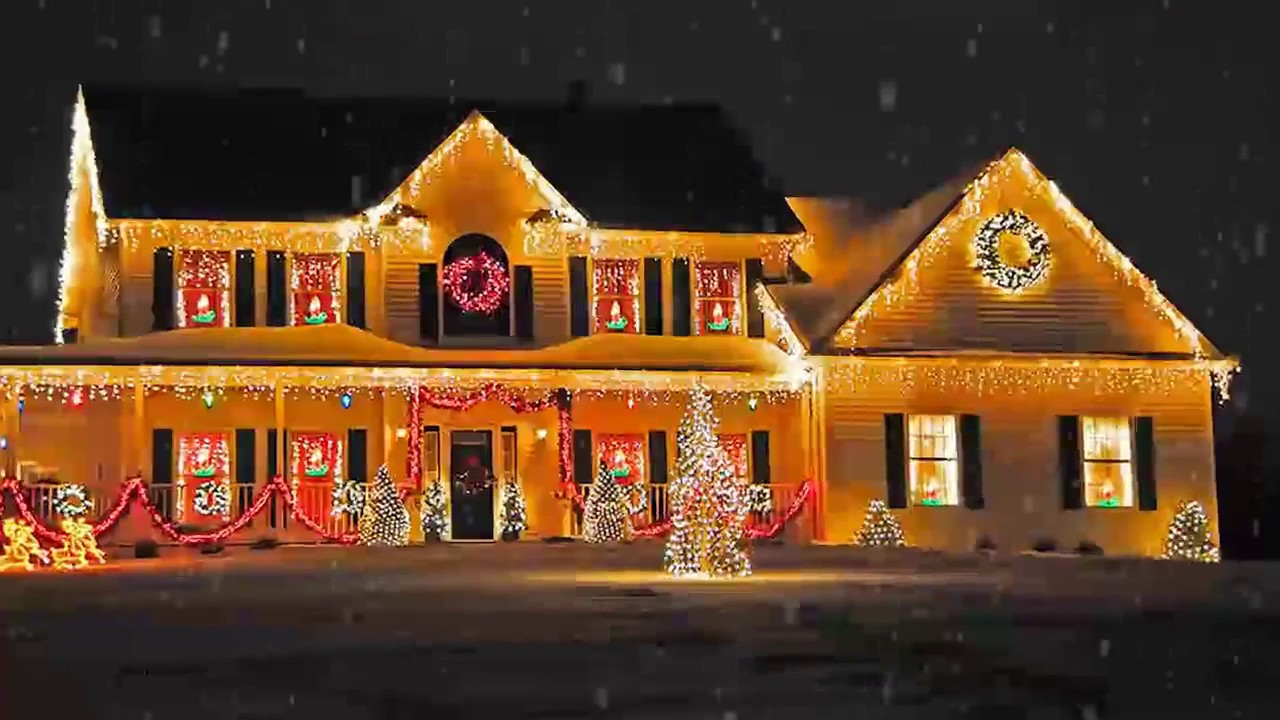
\includegraphics[scale=0.35]{figures/home_lightings.jpg}
	\caption{Пример внешнего домового освещения}
	\label{fig:subject:industry:example}
\end{figure}

Даже на фоне мирового финансового кризиса, а возможно, именно благодаря ему спрос на светодиодные источники света демонстрирует устойчивый рост по всему миру. Если еще 2–3 года назад светодиоды использовались преимущественно для вторичной декоративной подсветки, то в настоящее время технологии производства достигли того уровня, когда становится возможным их широкое применение и для функционального общего освещения.

Прогресс рынка общего освещения обусловлен двумя основными факторами. Первый — стремительный рост инвестиций в строительство в развивающихся странах. Второй — все большее внедрение дорогих технологий в освещение, включая светодиоды, что естественным образом повышает среднюю стоимость готовых осветительных приборов. Постоянно растет и рынок автомобильного освещения. В 2011 году его оборот оценивался примерно в 14 млрд евро, что составляет 20\% рынка освещения.

Так как рынок постоянно растет, сами товары совершенствуются и усложняются, то встает вопрос об управлении этими вещами. Контроллеров с маленькими дисплеями, либо просто кнопок переключения между анимациями теперь не хватает. Покупателям нужно куда больше функционала, плюс к тому, хорошо было бы иметь возможность постоянной поддержки системы управления, будь то ``патчи'' с исправлениями ошибок, либо добавление нового функционала. Для этого отлично подойдут устройства, которые и так у нас постоянно под рукой~--- мобильные телефоны. Сама же технология управления различными техническими устройствами с помощью мобильного телефона уже обзавелась названием ``Интернет вещей'' (англ. Internet of Things) или же коротко~-- IoT.

\subsection{Интернет вещей}
\label{sec:subject:iot}

Интернет вещей — концепция вычислительной сети физических предметов («вещей»), оснащённых встроенными технологиями для взаимодействия друг с другом или с внешней средой, рассматривающая организацию таких сетей как явление, способное перестроить экономические и общественные процессы, исключающее из части действий и операций необходимость участия человека \cite{wiki_iot}.

Концепция сформулирована в 1999 году как осмысление перспектив широкого применения средств радиочастотной идентификации для взаимодействия физических предметов между собой и с внешним окружением. Наполнение концепции «интернета вещей» многообразным технологическим содержанием и внедрение практических решений для её реализации начиная с 2010-х годов считается устойчивой тенденцией в информационных технологиях, прежде всего, благодаря повсеместному распространению беспроводных сетей, появлению облачных вычислений, развитию технологий межмашинного взаимодействия, началу активного перехода на IPv6 и освоению программно-конфигурируемых сетей \cite{wiki_iot}.

На 2017 год термин «Интернет вещей» распространяется не только на киберфизические системы для «домашнего» применения, но и на промышленные объекты. Развитие концепции «Интеллектуальных зданий» получило название «Building Internet of Things» (BIoT, «Интернет вещей в здании»), развитие распределённой сетевой инфраструктуры в АСУ ТП привело к появлению «Industrial Internet of Things» (IIoT, «Индустриальный (промышленный) интернет вещей») \cite{wiki_iot}.

Что представляет из себя интернет вещей:
\begin{itemize}
	\item постоянная поддержка человека предметами, которые его находятся рядом с ним;
	\item прозрачность процессов, ориентация на результат;
	\item это говорить не как надо делать, а что должно получиться.
\end{itemize}

Интернет вещей (IoT) – это, в основном, физические устройства: транспортные средства, бытовая техника, строительные материалы и другие предметы, взаимосвязанные между собой с целью сбора и обмена данными при помощи датчиков, программного обеспечения, проводов, микрочипов и прочей электроники через подключение к Сети (Интернет, Bluetooth).

Самоуправляемые автомобили, личные помощники, бытовая смарт-техника, энергосберегающие строительные материалы – этот список можно продолжать бесконечно. Все это влияющие на массы продукты, которые разрабатываются и развиваются для того, чтобы сделать жизнь проще, функциональнее, продуктивнее и эффективнее.

Согласно исследованиям компании Gartner, к прошлому году существовало 3.8 миллиардов соединенных между собой устройств: смарт-автомобили, детекторы дыма, дверные замки, промышленные роботы, уличные фонари, программы для мониторинга сердечного ритма, поезда, ветровые турбины, даже теннисные ракетки и тостеры.

По подсчетам компании, к 2020 г будет существовать 25 миллиардов смарт-девайсов, передающих крошечные объемы информации нам, в облако и обратно. Уходящий в отставку генеральный директор Cisco Джон Чамберс заявил, что в течение 5 лет будут существовать 50 миллиардов девайсов на сумму 19 триллионов долларов США. Говорят, что эти смарт-девайсы начинают приводить в действие четвертую промышленную революцию (после пара, электричества и проводных компьютеров).

~
\begin{figure}[H]
\centering
	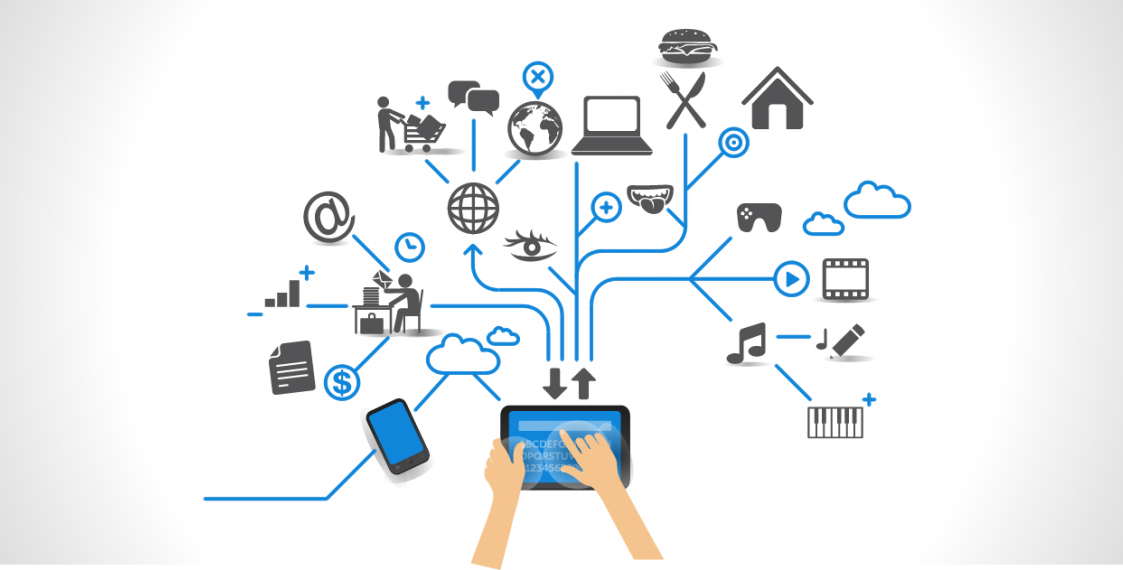
\includegraphics[scale=0.4]{figures/iot_scheme.png}
	\caption{Схематичное представление IoT}
	\label{fig:subject:iot:scheme}
\end{figure}

4 примера умных интернет вещей:
\begin{itemize}
	\item если вы уйдете из дома без кошелька, он сообщит вам об этом по телефону, а сенсор на ошейнике кота сообщит координаты,если кот сбежал далеко от дома;
	\item если вы забыли выключить утюг или телевизор, не нужно идти домой проверять: они сами доложат свой статус;
	\item когда закончился кофе или стиральный порошок, заказать его можно одним нажатием на кнопку;
	\item интернет-вещи напомнят, когда нужно поливать цветы, а целая система, подключенная к вашему огороду, подскажет, когда нужно полить грядки и включить поливающее оборудование.
\end{itemize}

Световое оборудование, описанное в данном дипломном проекте, поставляется вместе с мобильным приложением. Оно как раз подходит под описание продукта в Интернете вещей. Данные устройства (адресные светодиодные ленты), обладают wi-fi модулями для связи с мобильны приложением и получением команд от него, а также для связи с другими адресными светодиодными лентами. Само приложение обладает возможностью объединения адресных лент в группы, для последующего взаимодействия сразу с несколькими адресными светодиодными лентами (например при внешнем украшении дома).

\subsection{Рынок Интернета вещей в Беларуси}
\label{sec:subject:belarus}

В 2017 году мобильный оператор velcom получил разрешение на коммерческий запуск первой в Беларуси узкополосной сети NB-IoT, предназначенной для «интернета вещей». Государственная комиссия по радиочастотам (ГКРЧ) предоставила velcom возможность использовать часть ранее выделенного компании частотного диапазона.

Специалисты называют новую технологию революционной. Беларусь станет одной из первых стран в Европе, которая запустит сеть NB-IoT (Narrow Band Internet of Things). В ближайшем будущем она может найти применение в решении различных задач – от управления «умными» счетчиками и устройствами в доме до внедрения интеллектуальных систем городского масштаба.

ГКРЧ разрешило запустить сеть NB-IoT в диапазоне 900 МГц, который сейчас используется в основном для стандарта GSM. Для «интернета вещей» velcom задействует узкую полосу частот в 200 кГц, что не повлияет на работу действующих сетей.

Стандарт NB-IoT до 30 раз превосходит используемые сейчас технологии M2M-связи по уровню проникновения сигнала. В частности, им будут покрыты труднодоступные места, в том числе подвалы, низины и здания с толстыми стенами и перекрытиями. Новый стандарт также отличают широкая область применения, экономичность и энергоэффективность \cite{iot_belarus_velcom}.

В 2018 году российская компания \enquote{МТС} также получила разрешение от ГКРЧ на создание сети NB-IoT. Для создания новых продуктов доступны все частоты в диапазоне 900 МГц, предоставленные в соответствии с решением ГКРЧ.

МТС в своей сети продемонстрировал возможности NB-IoT впервые на выставке \enquote{ТИБО-2017} совместно с компанией Huawei: была развернута тестовая зона для создания новых продуктов и сервисов. Посетители убедились в достоинствах технологии на примере конкретных продуктов: сельскохозяйственной метеостанции, трекеров для детей и домашних животных, а также "умного" замка для пунктов проката велосипедов.

В мае 2019 года МТС провела тест международного роуминга в сети стандарта Narrowband IoT (NB-IoT).

Тест прошел успешно и подтвердил возможность бесперебойной работы и непрерывного обслуживания устройств NB-IoT в гостевой сети, сообщили в МТС. Теперь российская компания готова к полноценному запуску международного роуминга NB-IoT с другими операторами.

~
\begin{figure}[H]
\centering
	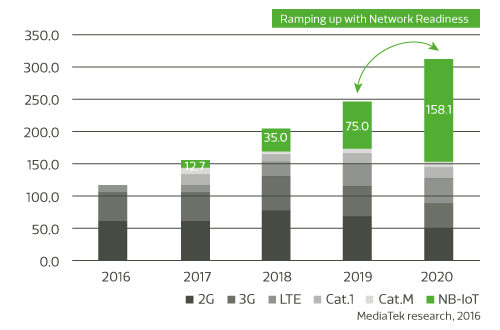
\includegraphics[scale=0.8]{figures/nbiotExample.png}
	\caption{Прогноз на распределение использования видов сотовой связи}
	\label{fig:subject:belarus:nbiot}
\end{figure}

Прогнозы таковы: в недалеком будущем большинство окружающих нас на работе и в быту вещей — от компьютера и смартфона до холодильника и фрезерного станка — будут связаны с интернетом и обмениваться с централизованным сервером или друг с другом информацией. Причем если к 2021 году количество обычных гаджетов вроде планшетов и умных телефонов увеличится до 8,7 млрд, то число IoT–устройств превысит 18 млрд. Свою пользу они будут доказывать в самых разных областях — от банального заказа холодильником недостающей еды в интернет–магазине (что фантастические фильмы предсказывали еще десятилетия назад) до полной автоматизации многих производств. Иначе говоря, условный робот–ремонтник сможет эффективно обслуживать информатизированный станок благодаря каналу связи между ними. Впрочем, заглядывать за горизонт событий совсем не обязательно: уже сегодня, допустим, БелАЗ использует IoT–концепцию и устанавливает датчики на свои большегрузы, чтобы в реальном времени отслеживать износ деталей и прогнозировать грядущий ремонт и закупку нужных запчастей \cite{iot_belarus_prog}.

\subsection{Интернет вещей и мобильные приложения}
\label{sec:subject:mobile}

Мобильное приложение~--- программное обеспечение, предназначенное для работы на смартфонах, планшетах и других мобильных устройствах. Многие мобильные приложения предустановлены на самом устройстве или могут быть загружены на него из онлайновых магазинов приложений, таких как App Store, BlackBerry App World, Google Play, 1mobile market, Windows Phone Store, Яндекс.store и других, бесплатно или за плату \cite{wiki_mobile_def}.

На сегодняшний день существует огромное количество разнообразных приложений, загружаемых в мобильный телефон. Все приложения можно условно разделить на развлекательные (игры, плееры, «читалки»), коммуникационные (мессенджеры, навигационные (карты), справочные (словари, базы данных) и прикладные (все от калькулятора до графических программ) \cite{mobile_business}.

Мобильные технологии имеют ряд неоспоримых преимуществ перед любыми другими видами маркетинговых коммуникаций. Использование в своем приложении функций игрового характера позволяет привлечь большую аудиторию, заинтересовав ее. Вы можете получать отзывы напрямую от своих клиентов, без посредников (таких, как интернет-сайты или ваши сотрудники) и прямо в момент совершения покупки.

Возможности мобильных приложений практически безграничны, но немало программ удаляются пользователем уже через пару суток после установки. Так что к разработке мобильного приложения стоит относиться серьезно и ответственно, как и к любому другому инструменту маркетинга.

В 2012 году рынок мобильных приложений оценивался в 53 миллиарда долларов, а прогноз на 2016 год гласил, что предполагаемый рост составит около 100 миллиардов долларов. Эти цифры немного отличаются у разных исследователей, но очевидным остается то, что мобильный рынок действительно масштабен. Доход разработчики получают с помощью внутренних in-app покупок, рекламы внутри приложений, а также сбора больших данных (big data). Самые многообещающие категории – это социальные сети, производительность, рекламные сервисы, а также полезные приложения для различных целей. Самые быстрорастущие рынки – Юго-Восточная Азия и Латинская Америка \cite{mobile_market}.

В США, 67~\% пользователей используют смартфон, чтобы выходить в интернет каждый день, и большинство никогда не выйдут из дома без своего телефона. Аналогичный рост использования смартфонов наблюдается и в России – даже пользователи с доходами ниже среднего чаще выбирают смартфон вместо компьютера, чтобы всегда оставаться на связи с миром. Исследования рынка показывают, что около половины всех пользователей мобильных телефонов загрузили приложения, а две трети из них регулярно их используют. Большинство пользователей мобильных приложений находятся в возрастном промежутке от 25 до 30 лет, женаты или замужем, живут в пригородных районах, и имеют высшее образование. Таким образом, пользователи мобильных приложений в целом моложе, более образованы и имеют более высокий доход, нежели пользователи, не использующие мобильные приложения \cite{mobile_market}.

Две операционные системы Android и iOS доминируют на мобильном рынке. У Apple и Google два самых популярных магазина приложений, и сегодня кажется, что другим участникам рынка можно даже не мечтать, чтобы пробиться к лидерству.

Есть интересная статистика среднемесячного дохода, который приносили мобильные приложения. Статистику привел иностранный Forbes. Итак, в 2013-м году iOS приносила своим разработчикам в среднем \$4 000 в месяц, на втором месте был Android с его \$1 125, и аутсайдером был Windows Phone и всего \$625 \cite{mobile_tendency}.

В 2016-м году ситуация поменялась. Согласно данным Statista, приложение Windows Phone приносит, в среднем, \$11 400 в месяц, тогда как приложение iOS генерирует \$8 100, а Android — \$4 900. При этом 75~\% разработчиков являются приверженцами Android \cite{mobile_tendency}.

Пользовательские приложения для Интернета вещей можно разделить на две большие группы по их назначению:
\begin{itemize}
    \item Приложения для сбора и анализа данных – их главная задача заключается в снятии показаний с устройства и сохранении их в приложении (приложения для фитнес-трекеров, весов, измерителей влажности, камер, нитратомеров и т.д.);
    \item Приложения для управления – они способны не только проследить за устройством, но и изменить его состояние (приложения для кофеварок, чайников, умного дома и т.д.).
\end{itemize}

Приложения, как и сами IoT устройства, можно отнести к какой-либо категории – «фитнес и здоровье», «медицина», «бытовая техника», «мультимедиа», «умный дом». Все зависит от того, каким устройством оно управляет. В любом случае, если этот девайс есть в продаже, то приложение к нему можно скачать в PlayMarket и AppStore абсолютно бесплатно. Обычно такие приложения очень просты в использовании, причем, как правило, одно приложение создается на всю линейку техники одного производителя, а пользователь уже синхронизирует те устройства, которые имеются у него. Конечно, можно загрузить данное приложение и без устройства, но в таком случае оно будет бесполезно, так как сразу потребует подключить к нему гаджет \cite{mobile_apps_iot}.

Рассмотрим функциональные возможности некоторых пользовательских IoT приложений. Многие «умные» устройства категории «фитнес и здоровье» отслеживают различные физиологические показатели организма. К примеру, глюкометр iHealth Smart Glucometer, разработанный компанией iHealth Labs Inc., может контролировать уровень сахара в крови и пересылать результаты измерений на смартфон, в приложение iHealth Gluco-Smart (Рисунок~\ref{fig:subject:mobile:iHealth}). Данные измерений могут быть сохранены в само устройство (около 500 измерений) или, если смартфон под рукой, сразу в мобильное приложение. Кроме того собранную информацию можно загрузить в облачное хранилище, предоставляемое пользователям бесплатно.

В данном приложении можно следить за изменением уровня сахара в течение дня, недели, месяца и т.д., контролировать срок годности тестовых полосок, устанавливать напоминания о необходимости измерений уровня сахара или приеме лекарств, отправлять статистику измерений (в виде графика или таблицы) на электронную почту или делиться результатами в социальных сетях. Информация передается на мобильное устройство по Bluetooth. К результатам измерений можно добавлять голосовые и текстовые заметки о питании, занятиях спортом, количестве углеводов в пище и многое другое \cite{mobile_apps_iot}.

~
\begin{figure}[H]
\centering
	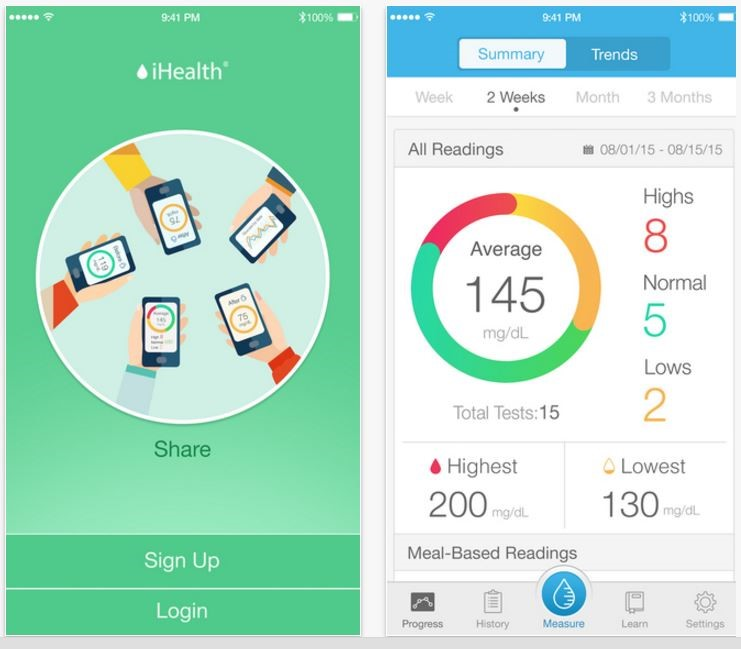
\includegraphics[scale=0.8]{figures/iHealth.jpg}
	\caption{Мобильное приложение для контроля уровня сахара}
	\label{fig:subject:mobile:iHealth}
\end{figure}

Все это говорит нам о том, что рынок мобильных приложений является очень перспективным и быстрорастущим. Мобильные приложения очень помогают в продвижении товара. Также они очень удобны как для пользователя, так и для разработчика, так как предоставляют большой спектр всевозможных датчиков и сетевых возможностей. Теперь понятно, что управление световым оборудованием с помощью именно мобильного приложения, это самый логичный и верный вариант для выбора вектора развития производства светового оборудования.

\subsection{Описание алгоритма калибровки гирлянды}
\label{sec:develop:algorithm}

При использовании гирлянды пользователь может повесить ее каким угодно образом. Однако при этом часть анимаций, которые расчитаны на конкретное расположение лампочек друг от друга, будут воспроизводится некорректно, представляя из себя мешанину из цветов. Алгоритм калибровки призван устранить данный недостаток анимаций. Пользователь с помощью камеры снимает небольшую анимацию на гирлянде, а потом алгоритм обрабатывает данные снимки и понимает расположение лампочек относительно друг друга.

\subsubsection{} Анимация калибровки
\label{sec:develop:algorithm:animation}

Анимация калибровки представляет собой последовательность из трех цветов (красный, синий и зеленый) для каждой лампочки. Ее суть заключается в том, что каждой лампочке задают определенную последовательность из трех цветов (адреса представляются в троичной системе исчисления). Последовательности при каждой калибровке генерируются заново, чтобы исключить проблему, когда рядом лежащие лампы горят одним цветом, что может привести к наслоению их друг на друга при обработке изображения. Пример изображен на рисунке~\ref{fig:develop:algorithm:animation}.

Шаги анимации:
\begin{itemize}
	\item все лампочки горят синим цветом~-- нужно, чтобы алгоритм понял, что анимация началась;
	\item все лампочки гаснут~-- алгоритм использует прошлый кадр с синими лампами и этот кадр, чтобы вычленить из всего изображения место, где будут находится лампы, отфильтровав все остальные предметы с синим, красным или зеленым цветом;
	\item последовательности цветов~-- алгоритм анимирует гирлянду в трех цветах. Количество цветов в последовательности вычисляется как $\lfloor\log_3 a\rfloor$, где $a$~-- количество лампочек в гирлянде.
\end{itemize}

~
\begin{figure}[H]
\centering
	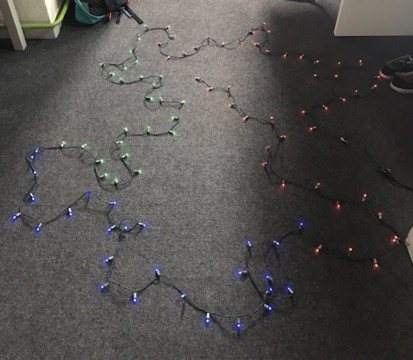
\includegraphics[scale=0.8]{figures/calibration_animation.jpg}
	\caption{Пример кадра анимации}
	\label{fig:develop:algorithm:animation}
\end{figure}

\subsubsection{} Ядро алгоритма
\label{sec:develop:algorithm:core}

База алгоритма основывается на распознании цвета пикселей изображений и на Connected-Component Labeling алгоритме. Его суть состоит в группировке одинаковых пикселей с помощью алгоритма поиска в глубину. Так как этот алгоритм предназначен для работы с изображениями только двух цветов, то нам надо превратить изображение, снятое с камеры телефона, в черно-белое. Использовать черно-белое изображение для распознания трех цветов одновременно не представляется возможным, поэтому для начала мы формируем три изображения для каждого из цветов отдельно, переводя изображение в черно-белое, где белым выделен нужный нам цвет (Рисунок~\ref{fig:develop:algorithm:colorFinding}).

~
\begin{figure}[H]
\centering
	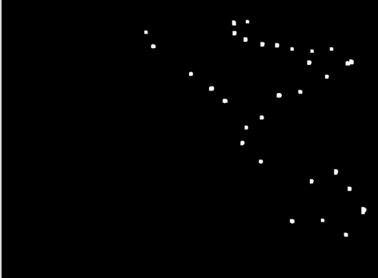
\includegraphics[scale=0.8]{figures/calibration_findedColor.jpg}
	\caption{Пример найденного цвета в кадре}
	\label{fig:develop:algorithm:colorFinding}
\end{figure}

Изображение может быть некачественным, поскольку оно сжимается для лучшей скорости работы; также еще стоит учитывать покачивания при съемке, засвет от других источников и тд. Следовательно, лампочка скорее всего будет состоять не из одной группы лежащих рядом пикселей, а из нескольких (Рисунок~\ref{fig:develop:algorithm:toBlackWhite}). Для этого применяется размытие по Гауссу вместе с фильтром по яркости (Рисунок~\ref{fig:develop:algorithm:blurring}). Далее находим группы из белых пикселей с помощью описанного выше CCL алгоритма (каждая группа - лампочка определенного цвета). При обработке всех кадров получаем последовательность из цветов с похожими координатами, так как это скорее всего одна и таже лампа, то группируем их в последовательность. Далее сопоставляем последовательность с уже заранее сгенерированными и находим адрес лампочки (Рисунок~\ref{fig:develop:algorithm:grouping}).

~
\begin{figure}[H]
\centering
	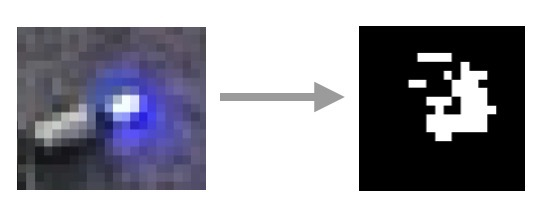
\includegraphics[scale=0.5]{figures/calibration_toBlackWhite.jpg}
	\caption{Первоначальное распознание цвета}
	\label{fig:develop:algorithm:toBlackWhite}
\end{figure}

~
\begin{figure}[H]
\centering
	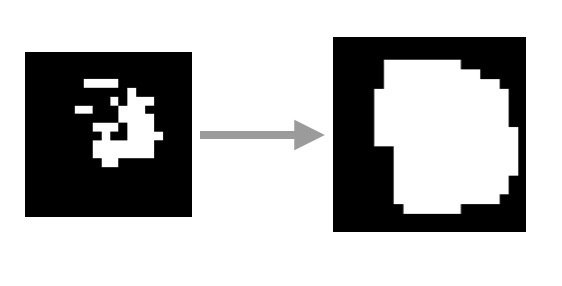
\includegraphics[scale=0.5]{figures/calibration_blurring.jpg}
	\caption{Распознание цвета после размытия}
	\label{fig:develop:algorithm:blurring}
\end{figure}

~
\begin{figure}[H]
\centering
	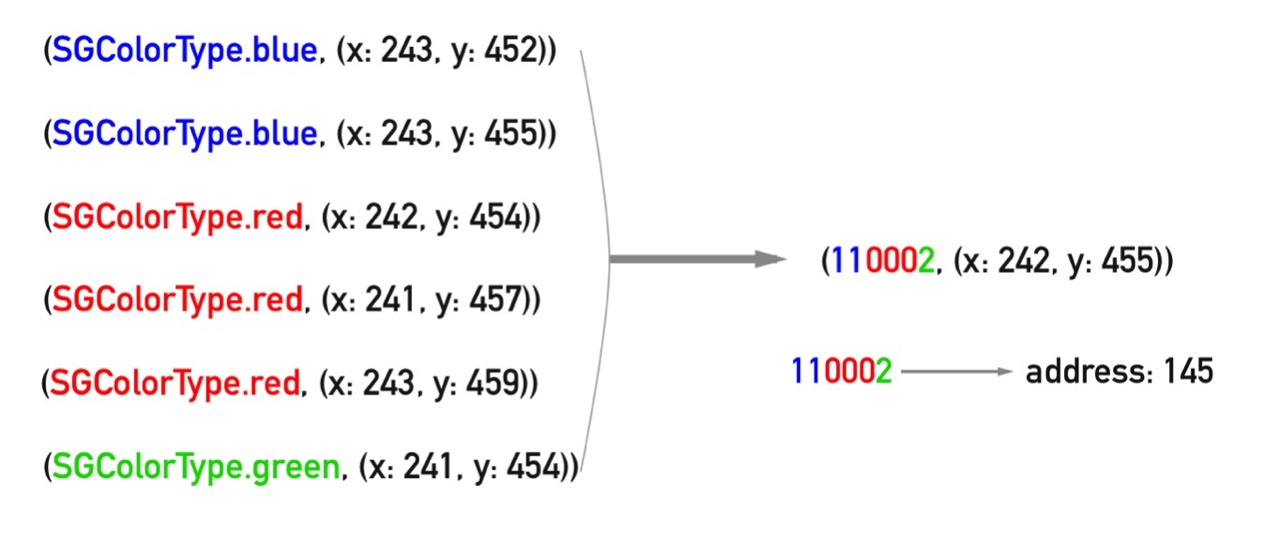
\includegraphics[scale=0.35]{figures/calibration_grouping.jpg}
	\caption{Пример группировки цветов по координатам}
	\label{fig:develop:algorithm:grouping}
\end{figure}

Сопоставление последовательности происходит следующим образом: сперва ищется точка с полностью совпадающей последовательностью цветов, если такой нет, то ищется последовательность отличающаяся на один цвет, потом на два и на три. Далее из всех найденных возможных точек, выбирается ближайшая к остальным уже найденным точкам.

\subsubsection{} Аппроксимация
\label{sec:develop:algorithm:approximation}

После обработки изображения часто остаются нераспознанными некоторые лампочки (обычно 20-30\%). Для устранения данной проблемы используется алгоритм аппроксимации. Он берет соседние найденные лампы возле ненайденных (например 63 и 69 лампочка, если алгоритм не нашел с 64 по 68 лампочку), строит между ними прямую и располагает на равноудаленных участках этого отрезка ненайденные лампочки. Если ненайденные лампочки находятся на концах гирлянды, то он просто строит примерно похожую линию и располагает гирлянды на ней. Это помогает построить примерно похожую гирлянду на экране телефона.

~
\begin{figure}[H]
\centering
	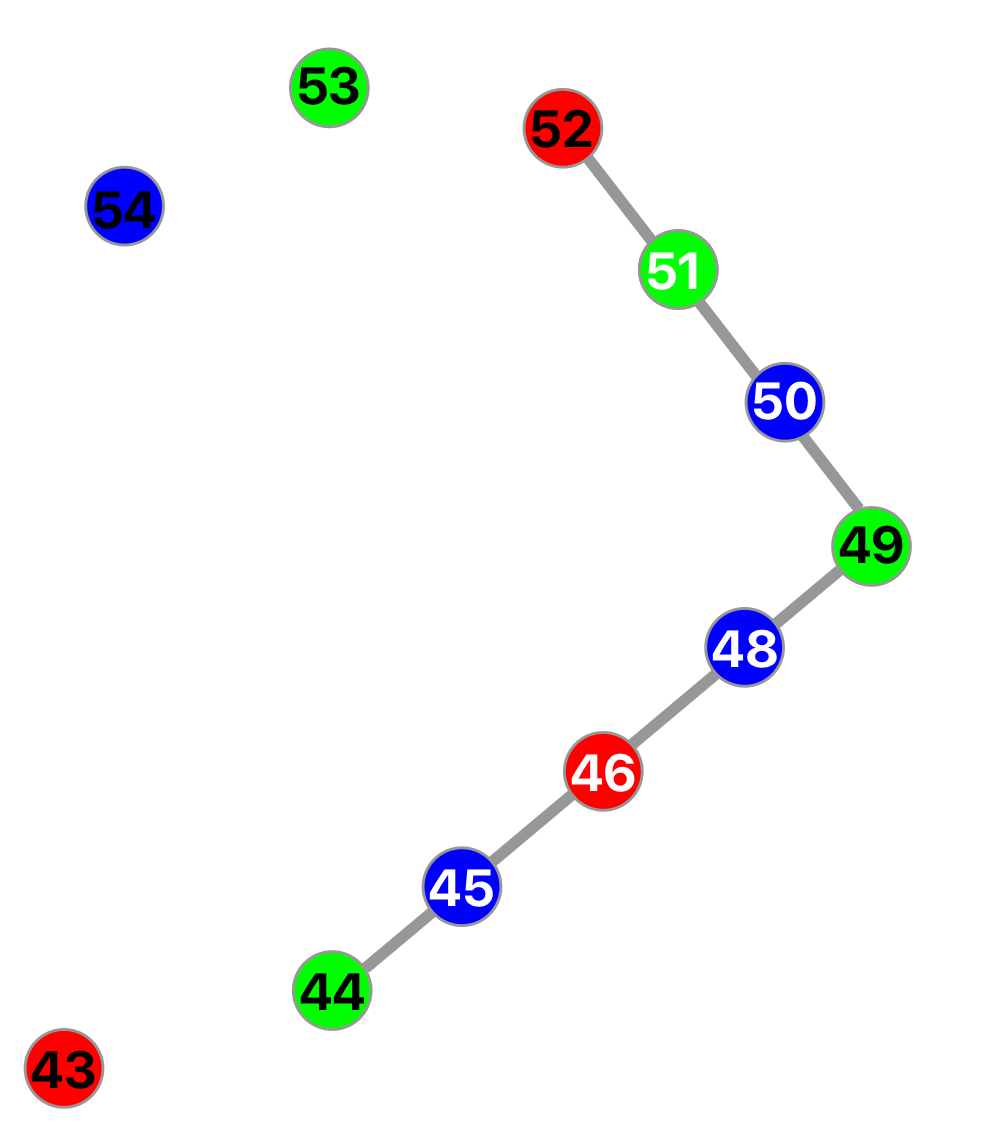
\includegraphics[scale=0.35]{figures/calibration_approximation.png}
	\caption{Пример работы аппроксимации (белым цветом отмечены аппроксимированные лампочки)}
	\label{fig:develop:algorithm:approximation}
\end{figure}

Итак, одним из главных требований для создания функционала по управлению адресной светодиодной лентой, является мобильное приложение. Мобильное приложение, в отличии от остальных видов программного обеспечения, позволяет наиболее полно и удобно для пользователя раскрыть потенциал Интернета вещей. На данный момент, мобильные устройства уже обладают сравнимой мощностью со стационарными компьютерами и позволяют работать со сложными и энергоёмкими алгоритмами, в том числе и с обработкой изображений.

Все это говорит о том, что производство мобильного приложения в паре с адресной светодиодной лентой является перспективным, в том числе и в финансовом плане.